\documentclass{article}

% Language setting
% Replace `english' with e.g. `spanish' to change the document language
\usepackage[english]{babel}

% Set page size and margins
% Replace `letterpaper' with `a4paper' for UK/EU standard size
\usepackage[letterpaper,top=2cm,bottom=2cm,left=3cm,right=3cm,marginparwidth=1.75cm]{geometry}

% Useful packages
\usepackage{amsmath}
\usepackage{graphicx}
\usepackage{float}
\graphicspath{{figure/}}
\usepackage[colorlinks=true, allcolors=blue]{hyperref}
\usepackage{ctex}
\usepackage{listings}
\usepackage{color}
\usepackage{xcolor}
\definecolor{dkgreen}{rgb}{0,0.6,0}
\definecolor{gray}{rgb}{0.5,0.5,0.5}
\definecolor{mauve}{rgb}{0.58,0,0.82}
\lstset{frame=tb,
     language=C++,
     aboveskip=3mm,
     belowskip=3mm,
     showstringspaces=false,
     columns=flexible,
     basicstyle = \ttfamily\small,
     numbers=left,
     numberstyle=\tiny\color{gray},
     keywordstyle=\color{blue},
     commentstyle=\color{dkgreen},
     stringstyle=\color{mauve},
     breaklines=true,
     breakatwhitespace=true,
     tabsize=4
}




\title{设计模式实验}
\author{刘恒星 2022229044}

\begin{document}
\maketitle

\section*{练习 1}

题目:在某 FPS (First - Person Shooting ,第一人称射击)游戏中提供了多个不同的游戏
场景。在每一个游戏场景中,提供了对应的地图(Map)、天气(Weather)和游戏背景音
乐(Sound)等。

请选择一种合适的设计模式对游戏场景进行设计,使得当用户选择游戏场景时,该场景
所对应的地图、天气和背景音乐能够同时出现;此外,还可以方便地在该游戏中增加新的游
戏场景。要求给出该设计模式的名称并结合实例绘制对应的结构图(即类图,类名、方法名
和属性名可自行定义)。


\vspace{1em}

答:应使用抽象工厂模式

\begin{figure}[H]
    \centering
    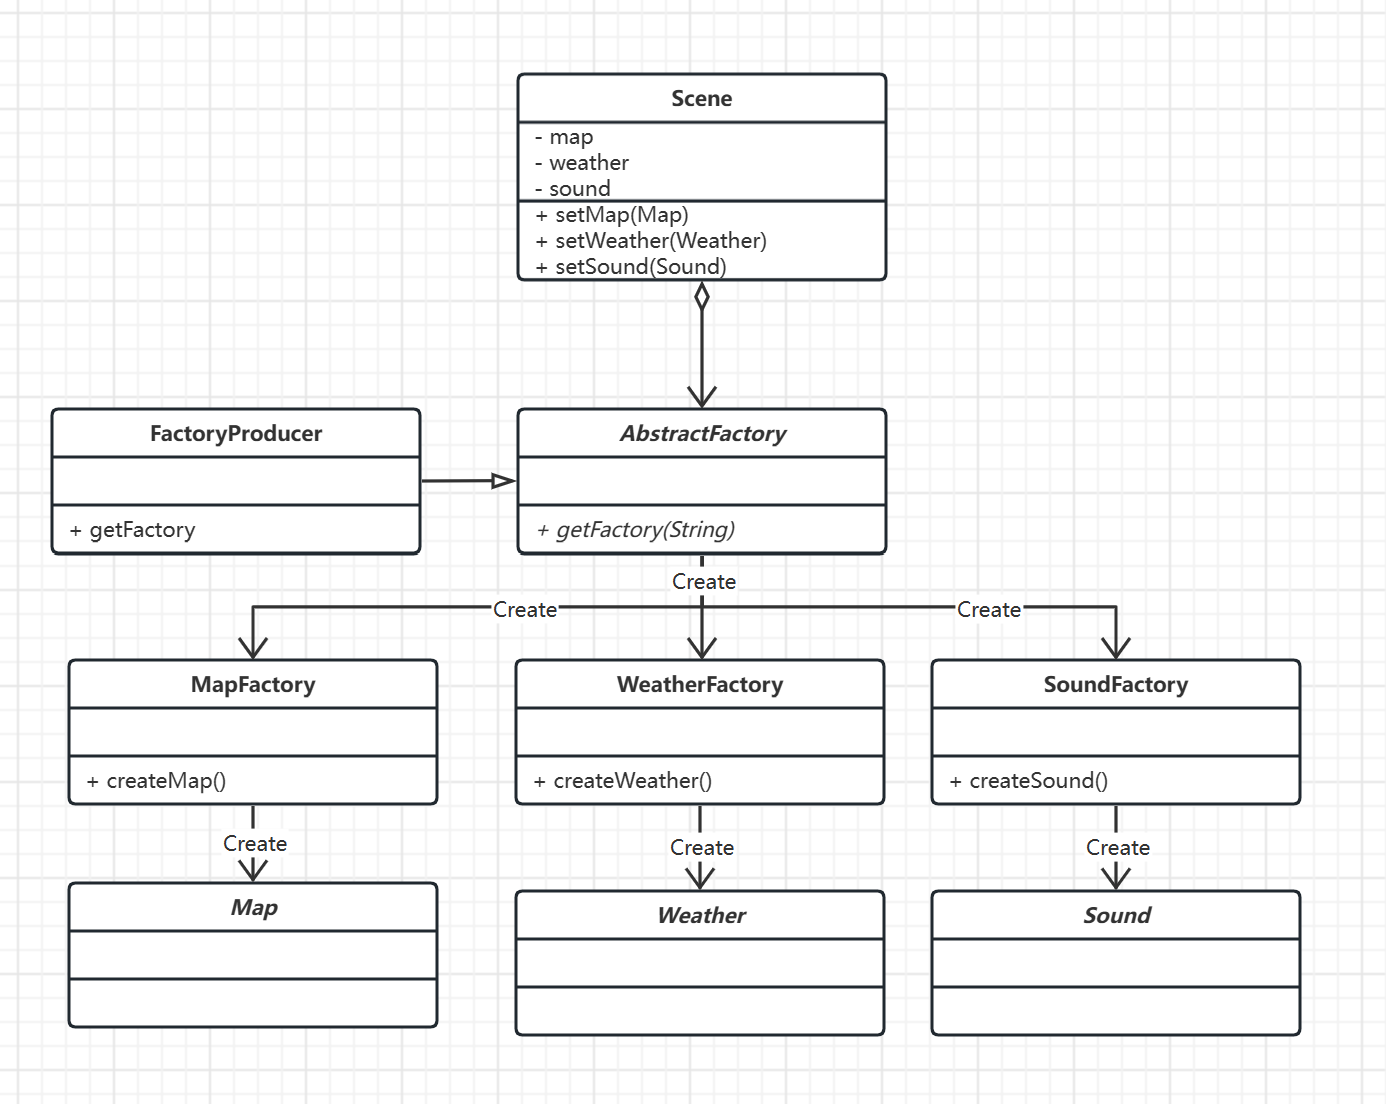
\includegraphics[width=0.9\textwidth]{UML1.png}
\end{figure} 



\section*{练习 2}

题目:在某 FPS 游戏中,系统可以给所有游戏成员发送通知,例如提示任务执行完毕、发送
新的任务提醒、发出敌人袭击警报等。

请选择一种合适的设计模式设计该系统通知模块,使得在系统中可以灵活地增加或删除
游戏成员。要求给出该设计模式的名称并结合实例绘制对应的结构图(即类图,类名、方法
名和属性名可自行定义)。

\vspace{1em}

答:应使用观察者模式,系统为被观察者,玩家为观察者,系统变化可以通知玩家,系统可以灵活添加和删除观察者

\begin{figure}[H]
    \centering
    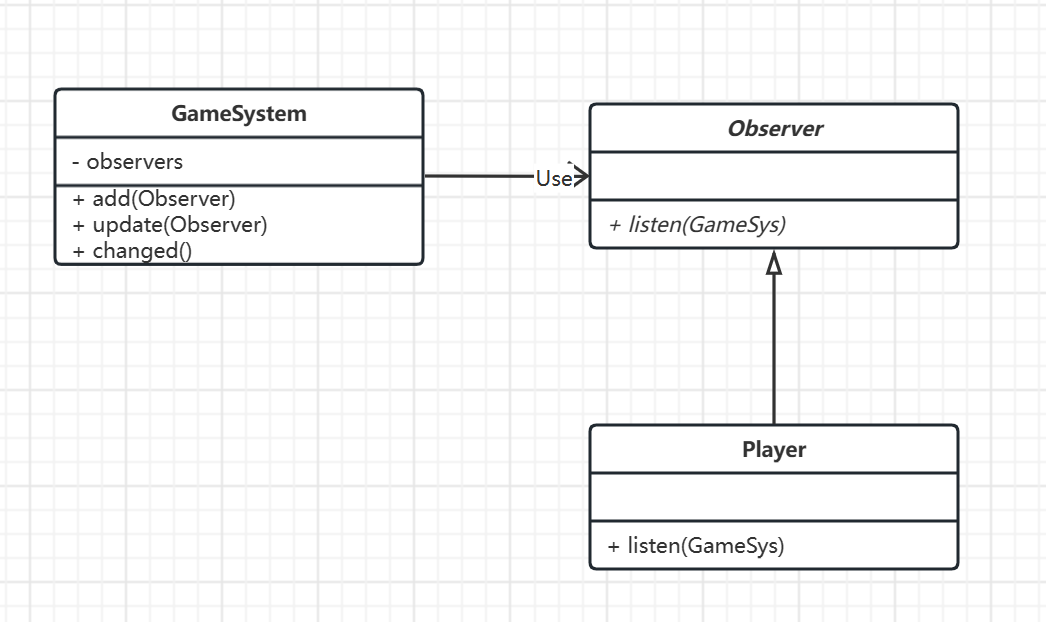
\includegraphics[width=0.9\textwidth]{UML2.png}
\end{figure} 


\section*{练习 3}

题目:某 FPS 游戏中提供了一个游戏管理器(Game Manager),通过该管理器用户可以对
音效(Sound Effect)、场景(Scene)、游戏角色(Role)等对象进行参数设置。为了节
约系统资源开且保证对象状态的一致性,在游戏运行时,用户只能打开唯一的一个管理器界
面。

根据以上描述,请选择两种合适的设计模式设计该游戏管理器,在实现对多个对象进行
统一设置的同时保证游戏管理器的唯一性。

要求给出这两种设计模式的名称并结合实例绘制对应的结构图(即类图,类名、方法么
和属性名可自行定义)。

\vspace{1em}

答:保证对象状态的一致性使用组合模式,保证管理器界面唯一性使用单例模式

\begin{figure}[H]
    \centering
    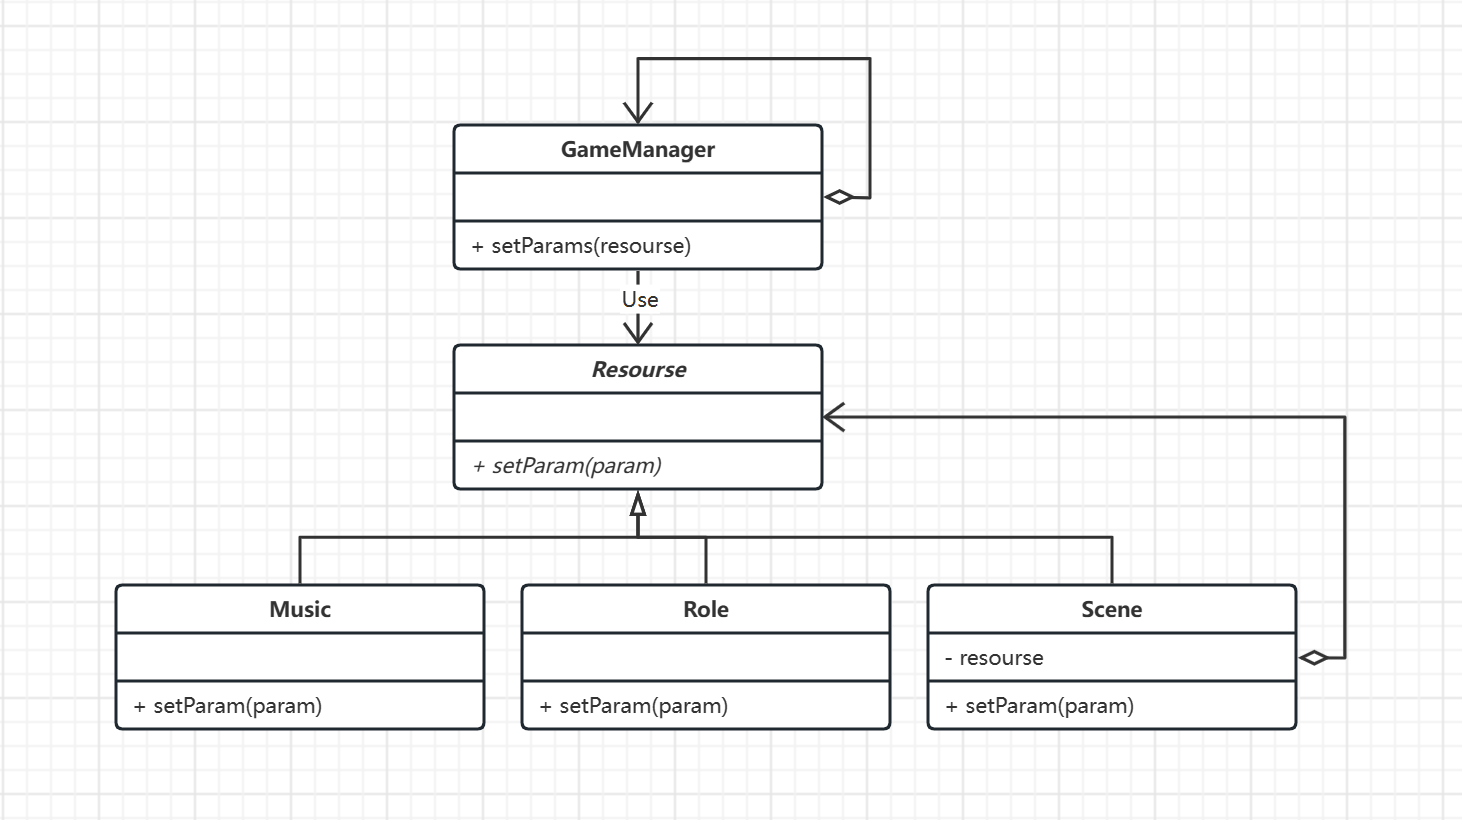
\includegraphics[width=0.9\textwidth]{UML3.png}
\end{figure} 


\section*{练习 4}

题目:为了让游戏场景呈现更加通真的效果,在某 FPS 游戏中可以对场景(Scene)的光照
效果等进行渲染(Rendering)。考虑到系统的可扩展性,开发人员可以实现表面渲染
(Surtace Rendering)和体渲染(Volume Rendering)等算法,也可以调用一些已有的渲
染引擎(Render Engine)中的渲染算法。在设计时需要考虑到渲染算法的可复用性,并能
够灵活地更换和增加新的渲染效果。

根据以上描述,请选择两种合适的设计模式设计该场景渲染模块,一方面证可以方便地
调用已有的渲染算法,另一方面还可以灵活地嵌人新的算法。

要求给出这两种设计模式的名称并结合实例绘制对应的结构图(即类图,类名、方法名
和属性名可自行定义)。

\vspace{1em}

答:考虑到可扩展性,使用装饰者模式。考虑到要调用已有的算法,可能会有不兼容的情况,所以使用适配器模式

\begin{figure}[H]
    \centering
    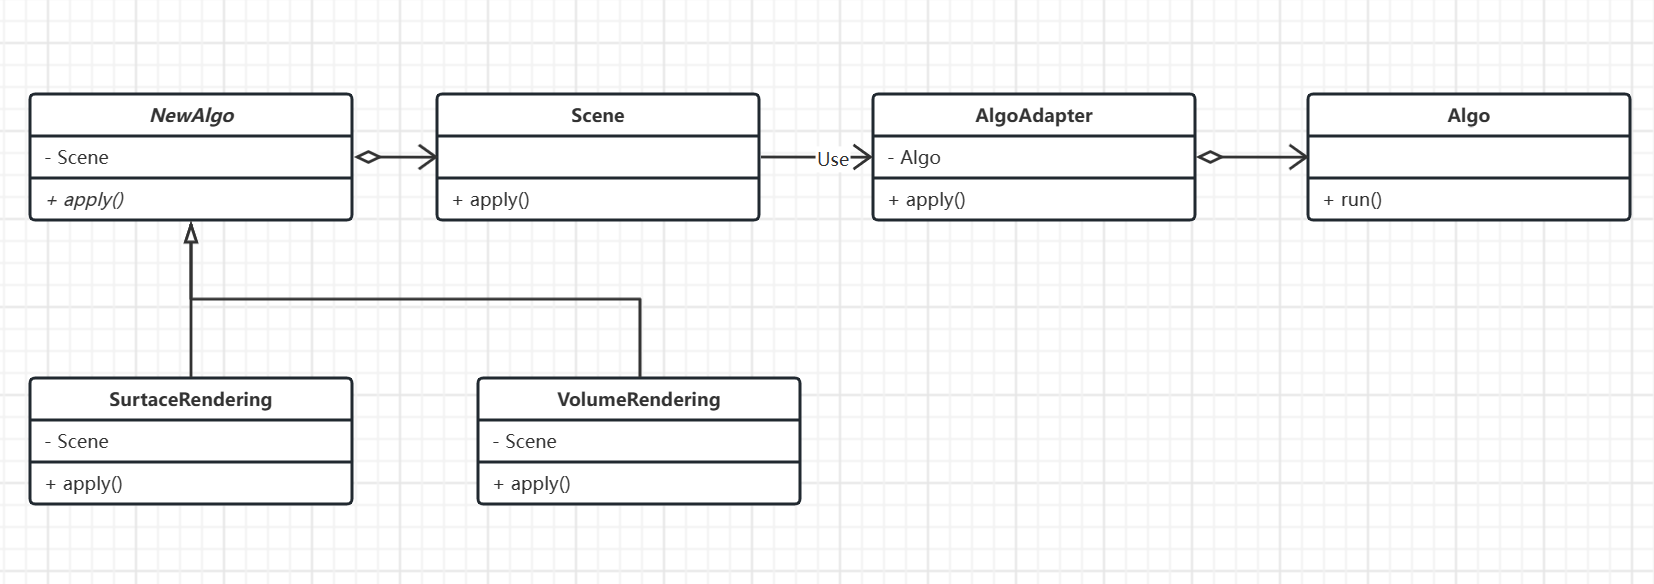
\includegraphics[width=0.9\textwidth]{UML4.png}
\end{figure} 


\section*{练习 5}

题目:In a First - Person Shooting (FPS) Game , a building or a blindage (掩体)is a 3D
structure that consists of many 3D Objects such as Cube (立方体), Cylinder (圆柱体), Pyramid (锥体) etc . When we fill a 3D block with color (such as Gray), the same color
also gets applied to the Objects in the block . Here a 3D block is made up of different
parts and they all have same operations . The parts of a 3D block can be small blocks .

Which design pattern can be used to implement the 3D structure ? Give the pattern’
s name and draw its structure diagram with this sample .

\vspace{1em}

答:涂色的时候对于block和组成block的组件都要涂色,具有一致性,所以使用组合模式

\begin{figure}[H]
    \centering
    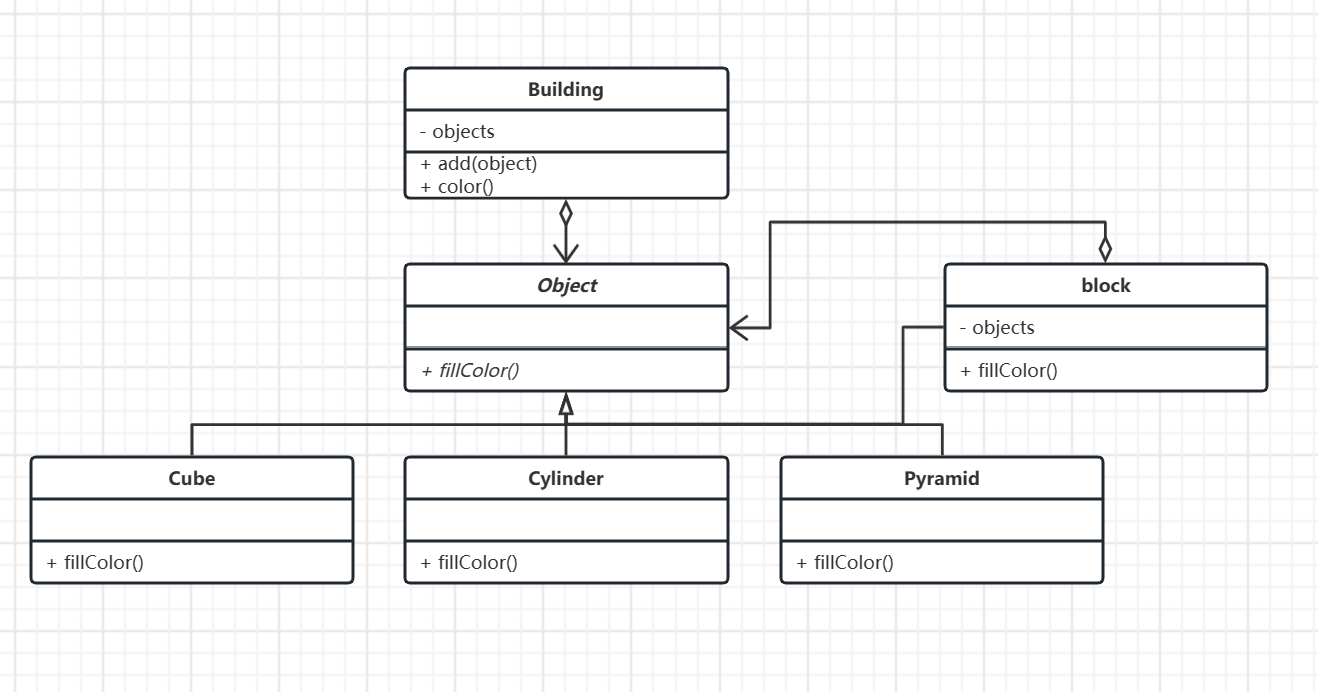
\includegraphics[width=0.9\textwidth]{UML5.png}
\end{figure} 






\end{document}